
\documentclass[nooutcomes]{ximera}
%\documentclass[space,handout,nooutcomes]{ximera}

% For preamble materials

\usepackage{pgf,tikz}
\usepackage{mathrsfs}
\usetikzlibrary{arrows}
\usepackage{framed}
\usepackage{amsmath}
%\pgfplotsset{compat=1.16}

\graphicspath{
  {./}
  {algorithms/}
  {../algorithms/}
}

\pdfOnly{\renewenvironment{image}[1][]{\begin{center}}{\end{center}}}

%%% This set of code is all of our user defined commands
\newcommand{\bysame}{\mbox{\rule{3em}{.4pt}}\,}
\newcommand{\N}{\mathbb N}
\newcommand{\C}{\mathbb C}
\newcommand{\W}{\mathbb W}
\newcommand{\Z}{\mathbb Z}
\newcommand{\Q}{\mathbb Q}
\newcommand{\R}{\mathbb R}
\newcommand{\A}{\mathbb A}
\newcommand{\D}{\mathcal D}
\newcommand{\F}{\mathcal F}
\newcommand{\ph}{\varphi}
\newcommand{\ep}{\varepsilon}
\newcommand{\aph}{\alpha}
\newcommand{\QM}{\begin{center}{\huge\textbf{?}}\end{center}}

\renewcommand{\le}{\leqslant}
\renewcommand{\ge}{\geqslant}
\renewcommand{\a}{\wedge}
\renewcommand{\v}{\vee}
\renewcommand{\l}{\ell}
\newcommand{\mat}{\mathsf}
\renewcommand{\vec}{\mathbf}
\renewcommand{\subset}{\subseteq}
\renewcommand{\supset}{\supseteq}
\renewcommand{\emptyset}{\varnothing}
\newcommand{\xto}{\xrightarrow}
\renewcommand{\qedsymbol}{$\blacksquare$}
\newcommand{\bibname}{References and Further Reading}
\renewcommand{\bar}{\protect\overline}
\renewcommand{\hat}{\protect\widehat}
\renewcommand{\tilde}{\widetilde}
\newcommand{\tri}{\triangle}
\newcommand{\minipad}{\vspace{1ex}}
\newcommand{\leftexp}[2]{{\vphantom{#2}}^{#1}{#2}}

%% More user defined commands
\renewcommand{\epsilon}{\varepsilon}
\renewcommand{\theta}{\vartheta} %% only for kmath
\renewcommand{\l}{\ell}
\renewcommand{\d}{\, d}
\newcommand{\ddx}{\frac{d}{dx}}
\newcommand{\dydx}{\frac{dy}{dx}}


\usepackage{bigstrut}


\newenvironment{sectionOutcomes}{}{}

\usepackage{array}
%\setlength{\extrarowheight}{-.2cm}   % Commented out by Findell to fix table headings.  Was this for typesetting division?  
\newdimen\digitwidth
\settowidth\digitwidth{9}
\def~{\hspace{\digitwidth}}
\def\divrule#1#2{
\noalign{\moveright#1\digitwidth
\vbox{\hrule width#2\digitwidth}}}


\title{Functions and Sequences}
\author{Bart Snapp and Brad Findell and Jenny Sheldon}
\begin{document}
\begin{abstract}
Problems about functions and sequences.
\end{abstract}
\maketitle


%\begin{problem}
%Problem
%\begin{freeResponse}
%\begin{hint}
%Hint
%\end{hint}
%\end{freeResponse}
%\end{problem} 

%
%Function given by graph
%Function given by recursive formula
%Function given by table
%Function given by complicated formula
%

\begin{problem}
A \textbf{sequence} is a function with a domain that is a subset of the $\answer[format=string]{integers}$.  

An \textbf{arithmetic sequence} is a(n) $\answer[format=string]{linear}$ function. 

A \textbf{geometric sequence} is a(n) $\answer[format=string]{exponential}$ function. 
\end{problem}

\begin{problem}
Suppose 

\end{problem}



\begin{problem}
The \textbf{$3n+1$ problem} involves integer sequences defined as follows:  Start with any positive integer. Then, if the current term is even, the next term is one half of the current term. If the current term is odd, the next term is $3$ times the current term plus $1$. 

Suppose the first term is 3.  Find the next several terms.  

\[
3, \answer{10}, \answer{5}, \answer{16}, \answer{8}, \answer{4}, \answer{2}, \answer{1}, \answer{4}, \answer{2}, \answer{1}.  
\]

Note that once the sequence reaches $1$, it cycles back to 1 repeatedly.  
\begin{problem}
If we use function notation to describe the sequence, then the recursive rule may be stated as follows: 

\begin{itemize}
\item If $f(k)$ is even, then $f(k+1) = \answer{f(k)/2}$. 
\item If $f(k)$ is odd, then $f(k+1) = \answer{3f(k) + 1}$.  
\end{itemize}

And given $f(1)=3$, it follows that $f(2)=\answer{10}$, $f(3)=\answer{5}$, and so on.  

Claim: No matter the initial (positive integer) value, the sequence will always reach 1.  

This claim is often called the Collatz Conjecture, in honor of Lothar Collatz, who introduced the idea in 1937.  As of 2020, the conjecture has been checked by computer for all starting values up to $2^{68} \approx 2.95\times 10^{20}$. The statement is still a conjecture (rather than a theorem) because no one has been able to prove that it holds for \textbf{all} possible initial values.  For more information, see \link[Wikipedia]{https://en.wikipedia.org/wiki/Collatz_conjecture}. 

\end{problem}

\end{problem}



\begin{problem}


A Actual (read from the graph or table or computed from a formula)
E Estimate (estimated from the graph or table or formula)

Interpolate vs. extrapolate 

M Model

NA not available (we don't have actual data, and our data is insufficient for a good estimate), 
DNE does not exist 



Columbus, Ohio State University Airport (KOSU)

Lat: $40.08^\circ$N, Lon: $83.08^\circ$W, Elev: $902$ ft.

\begin{tabular}{|c|c|c|}
\hline
Date  &   \multicolumn{1}{p{1.5cm}|}{\centering Time \\ (EDT)}  
      &   \multicolumn{1}{p{1.5cm}|}{\centering Temp. \\ ($^\circ $F)} \\ \hline
%10/29/21   &  10:53  &  58 \\
%             &  11:53  &  57 \\
%             &  12:53  &  58 \\
%             &  13:53  &  60 \\
%             &  14:53  &  60 \\
%             &  15:53  &  59 \\
%             &  16:53  &  58 \\
%             &  17:53  &  57 \\
%             &  18:53  &  57 \\
%             &  19:53  &  57 \\
%             &  20:53  &  57 \\
%             &  21:53  &  57 \\
%             &  22:53  &  56 \\
%             &  23:53  &  56 \\ \hline
%10/30/21   &  0:53  &  56 \\
%             &  1:53  &  56 \\
%             &  2:53  &  55 \\
%             &  3:53  &  55 \\
%             &  4:53  &  55 \\
%             &  5:53  &  55 \\
%             &  6:53  &  55 \\
%             &  7:53  &  55 \\
%             &  8:53  &  55 \\
%             &  9:53  &  55 \\
%             &  10:53  &  56 \\
%             &  11:53  &  58 \\
%             &  12:53  &  60 \\
%             &  13:53  &  59 \\
%             &  14:53  &  59 \\
%             &  15:53  &  59 \\
%             &  16:53  &  59 \\
%             &  17:53  &  56 \\
%             &  18:53  &  56 \\
%             &  19:53  &  56 \\
%             &  20:53  &  55 \\
%             &  21:53  &  54 \\
%             &  22:53  &  53 \\
%             &  23:53  &  53 \\ \hline
10/31/21   &  0:53  &  53 \\
             &  1:53  &  53 \\
             &  2:53  &  53 \\
             &  3:53  &  52 \\
             &  4:53  &  52 \\
             &  5:53  &  52 \\
             &  6:53  &  52 \\
             &  7:53  &  52 \\
             &  8:53  &  53 \\
             &  9:53  &  53 \\
             &  10:53  &  55 \\
             &  11:53  &  55 \\
             &  12:53  &  56 \\
             &  13:53  &  58 \\
             &  14:53  &  59 \\
             &  15:53  &  59 \\
             &  16:53  &  61 \\
%             &  17:53  &  60 \\
%             &  18:53  &  59 \\
%             &  19:53  &  58 \\
%             &  20:53  &  56 \\
%             &  21:53  &  55 \\
%             &  22:53  &  53 \\
%             &  23:53  &  52 \\
%11/01/21   &  0:53  &  51 \\
%             &  1:53  &  47 \\
%             &  2:53  &  44 \\
%             &  3:53  &  43 \\
%             &  4:53  &  42 \\
%             &  5:53  &  40 \\
%             &  6:53  &  39 \\
%             &  7:53  &  38 \\
%             &  8:53  &  40 \\
%             &  9:53  &  46 \\
\hline
\end{tabular}\qquad
\begin{tabular}{|c|c|c|}
\hline
Date  &   \multicolumn{1}{p{1.5cm}|}{\centering Time \\ (EDT)}  
      &   \multicolumn{1}{p{1.5cm}|}{\centering Temp. \\ ($^\circ $F)} \\ \hline
10/31/21     &  17:53  &  60 \\
             &  18:53  &  59 \\
             &  19:53  &  58 \\
             &  20:53  &  56 \\
             &  21:53  &  55 \\
             &  22:53  &  53 \\
             &  23:53  &  52 \\
11/01/21   &  0:53  &  51 \\
             &  1:53  &  47 \\
             &  2:53  &  44 \\
             &  3:53  &  43 \\
             &  4:53  &  42 \\
             &  5:53  &  40 \\
             &  6:53  &  39 \\
             &  7:53  &  38 \\
             &  8:53  &  40 \\
             &  9:53  &  46 \\
\hline
\end{tabular}


Let $F(t)$ denote the temperature (in degrees Fahrenheit) $t$ hours after the beginning of November.  

Note that the hourly readings all occur at $53$ minutes after the hour.  For ease of entry, we are going to take 53 minutes as 0.9 hours (though, in fact, 0.9 hours is exactly $\answer{54}$ minutes).  This minor simplification, allows us to write, for example, $F(0.9) = \answer{51}$, $F(1.9)=\answer{47}$, and $F(8.9)=\answer{40}$.  

From real-world data, it is often reasonable to estimate values that are not directly available.  In particular, to \textbf{interpolate} is to estimate between available data values, and to \textbf{extrapolate} is to estimate beyond available values.  
\end{problem}


\begin{problem}
The following table shows a temperature forecast for the OSU Airport.  
\begin{image}
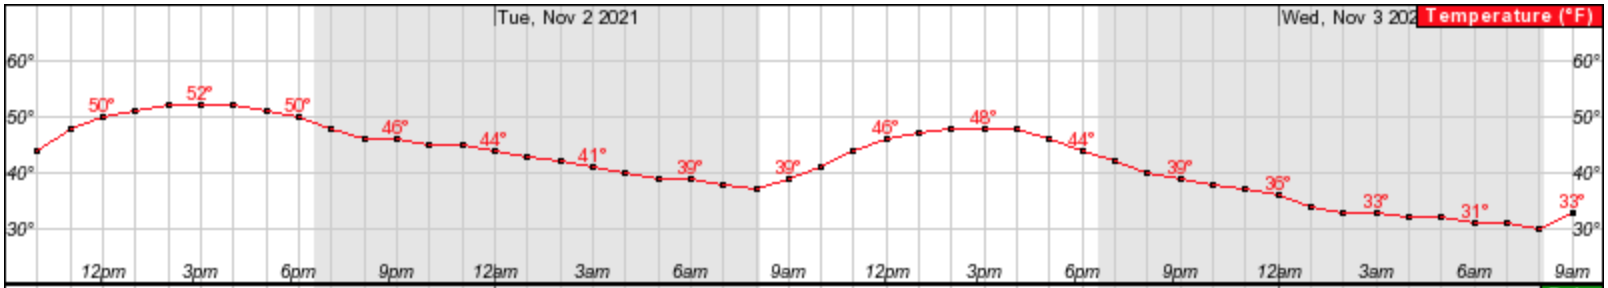
\includegraphics[scale=0.5]{columbusTemp.png}
\end{image}
Let $F(t)$ denote the predicted temperature (in degrees Fahrenheit) $t$ hours after the beginning of November (i.e., one minute before 12:01 am, 11/01/2021).  
\end{problem}

\end{document}



